\documentclass[12pt]{article}
\usepackage[T1]{fontenc}
\usepackage[light,math]{iwona}
\usepackage[latin1]{inputenc}
\usepackage{amsmath}
\usepackage{mathtools}
\usepackage{xspace}
\usepackage{graphicx}
\usepackage[english]{babel}
\usepackage[font=small,labelfont=bf]{caption}
\usepackage[centering,includeheadfoot,margin=2cm]{geometry}
\usepackage{tikz}
\usetikzlibrary{calc,shapes,arrows,automata,trees,shadows,decorations.pathmorphing,positioning,shapes.misc,shapes.arrows,chains,matrix,scopes,decorations.pathmorphing}
\begin{document}
\title{CS375 WK7}
\author{Jason N Mansfield}
\maketitle
%tikz terminal
\tikzset{
  nonterminal/.style={
    % The shape:
    rounded rectangle,
    % The size:
    minimum size=6mm,
    % The border:
    very thick,
    draw=red!50!black!50,         % 50% red and 50% black,
                                  % and that mixed with 50% white
    % The filling:
    top color=white,              % a shading that is white at the top...
    bottom color=red!50!black!20, % and something else at the bottom
    % Font
    font=\itshape
  },
  terminal/.style={
    % The shape:
    diamond,
    minimum size=6mm,
    % The rest
    very thick,draw=black!50,
    top color=white,bottom color=orange!20,
    font=\ttfamily},
  skip loop/.style={to path={-- ++(0,#1) -| (\tikztotarget)}}
}

{
  \tikzset{terminal/.append style={text height=1.5ex,text depth=.25ex}}
  \tikzset{nonterminal/.append style={text height=1.5ex,text depth=.25ex}}
}
%end of tikz terminal stuff

\begin{figure}
\begin{center}
\caption{Q01: FA}
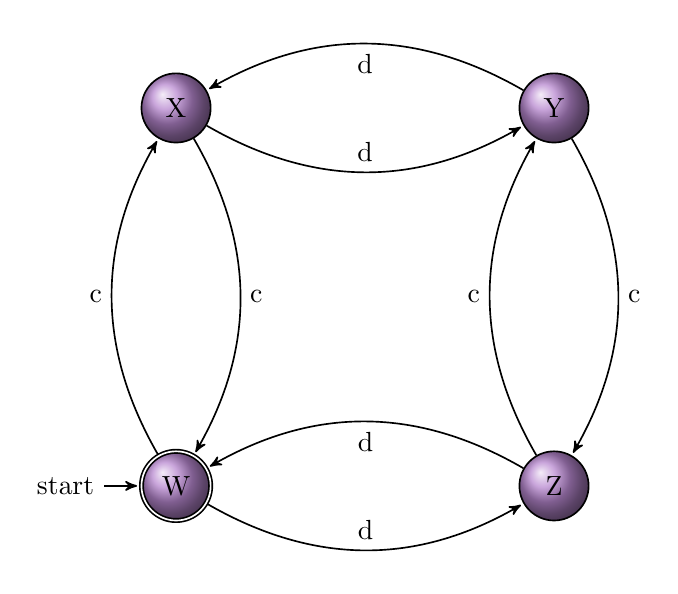
\begin{tikzpicture}[->,>=stealth',shorten >=1pt,auto,node distance=4.8cm, semithick]
\tikzstyle{every state}=[draw=black,text=black, ball color=red!40!blue!47!]
\node[state] (X) {X};
\node[state][right of=X](Y){Y};
\node[state,initial,accepting][below of=X](W){W};
\node[state][below of=Y](Z){Z};
\path (X)edge [bend right] node{d}(Y)
              edge [bend left] node{c}(W)
          (Y)edge [bend right]node{d}(X)
              edge [bend left]node{c}(Z)
          (W)edge [bend left]node{c}(X)
               edge[bend right]node{d}(Z)
          (Z)edge[bend left]node{c}(Y)
              edge[bend right]node{d}(W);      
\end{tikzpicture} 
\end{center}
\end{figure}

\begin{figure}
\begin{tikzpicture}[
        point/.style={coordinate},>=stealth',thick,draw=black!50,
        tip/.style={->,shorten >=0.007pt},every join/.style={rounded corners},
        hv path/.style={to path={-| (\tikztotarget)}},
        vh path/.style={to path={|- (\tikztotarget)}},
        text height=1.5ex,text depth=.25ex % align text horizontally
    ]
    
   \node (start)   [nonterminal]                        {START};
   \node (reject)   [nonterminal]                        {REJECT};
   \node (read) [terminal,right=of start]           {digit};
   \node (accept)     [nonterminal,right=of read]         {ACCEPT};
   \path (start)   edge[->] (read)  %  simple edges
             (read) edge[->] (accept);
   \draw [->]
     %  start right of digit.east, that is, at the point that is the
     %  linear combination of digit.east and the vector (2mm,0pt). We
     %  use the ($ ... $) notation for computing linear combinations
     ($ (read.east) + (2mm,0) $)
     %  Now go down
     -- ++(0,-1.1)
     %  And back to the left of digit.west
     -| ($ (read.west) - (2mm,0) $);
\end{tikzpicture}

\end{figure}




\end{document}